\documentclass[12pt, twoside]{article}
\documentclass[12pt, twoside]{article}
\usepackage[letterpaper, margin=1in, headsep=0.2in]{geometry}
\setlength{\headheight}{0.6in}
%\usepackage[english]{babel}
\usepackage[utf8]{inputenc}
\usepackage{microtype}
\usepackage{amsmath}
\usepackage{amssymb}
%\usepackage{amsfonts}
\usepackage{siunitx} %units in math. eg 20\milli\meter
\usepackage{yhmath} % for arcs, overparenth command
\usepackage{tikz} %graphics
\usetikzlibrary{quotes, angles}
\usepackage{graphicx} %consider setting \graphicspath{{images/}}
\usepackage{parskip} %no paragraph indent
\usepackage{enumitem}
\usepackage{multicol}
\usepackage{venndiagram}

\usepackage{fancyhdr}
\pagestyle{fancy}
\fancyhf{}
\renewcommand{\headrulewidth}{0pt} % disable the underline of the header
\raggedbottom
\hfuzz=2mm %suppresses overfull box warnings

\usepackage{hyperref}
\usepackage{float}

\title{Algebra 2}
\author{Chris Huson}
\date{May 2024}

\fancyhead[LE]{\thepage}
\fancyhead[RO]{\thepage \\ Name: \hspace{1.5cm} \,\\}
\fancyhead[LO]{BECA/Huson/Algebra 2: Regents Preparation \\* 30 May 2024}

\begin{document}

\subsubsection*{Prep \#20: Normal distributions}
\begin{enumerate}[itemsep=0.5cm]
\item A population is normally distributed with a mean of 100 and a standard deviation of 10. Find the proportion of the population that falls above 110, to the \emph{nearest thousandth}. \vspace{3cm}

\item The distribution of the diameters of ball bearings made under a given manufacturing process is normally distributed with a mean of 4 cm and a standard deviation of 0.2 cm. What proportion of the ball bearings will have a diameter less than 3.7 cm?\vspace{4cm}

\item There are 440 students at Thomas Paine High School enrolled in U.S. History. On the April report card, the students' grades are approximately normally distributed with a mean of 79 and a standard deviation of 7. Students who earn a grade less than or equal to 64.9 must attend summer school. (sketch and label the distribution)  \begin{enumerate}
    \item Calculate the number of standard deviations the 64.9 cutoff score is from the mean. \vspace{1cm}
    \item What percentage of the students scored at or below 64.9? \vspace{2cm}
    \item Find the number of students who must attend summer school for U.S. History rounded to the \emph{nearest whole} student.
\end{enumerate} \vspace{2cm}


\newpage
\item Graph the function $f(x) = x^4-2x^{3}-5x^{2}+3x+4$. 
\begin{center}
    \begin{tikzpicture}[scale=0.65]
        \draw[lightgray,very thin] (-10,-10) grid (10,10);
        \draw [thick,<->] (-10.5,0)--(10.5,0) node [right] {$x$};
        \draw [thick,<->] (0,-10.5)--(0,10.5) node [above] {$f(x)$};
        \foreach \x in {2}
            \draw[thick] (\x cm,5pt) -- (\x cm,-5pt) node[below] {$1$};
        \foreach \y in {2}
            \draw[thick] (4pt,\y cm)--(-4pt,\y cm) node[left]{10};
    \end{tikzpicture}
    \end{center}
Mark and label the zeros of the function to the \emph{nearest hundredth}. \\[2cm]
Describe the behavior of the given function as $x$ approaches positive infinity.


\end{enumerate}
\end{document}